\chapter
 [Preliminaries]
 {Preliminaries}
\label{chp:background}

\reminder{Status: mostly copied from intro/background sections from paper chapters.
Still to do a final edit.}


\section{Quantum networks}
A quantum network consists of devices that are connected together and that can establish entanglement between separate devices in that network.
More specifically, we assume quantum network to consist of \textit{nodes} that are connected by \textit{classical channels} and \textit{quantum channels} (\cref{fig:network_model}).
Classical channels enable classical communication between nodes, while quantum channels are used for \textit{entanglement} generation between nodes.
Some of these devices are repeater nodes, assisting in long-distance entanglement generation.
So-called \textit{end nodes} (or \textit{processing nodes}, and hereafter called just `nodes') can be seen as quantum computers:
they contain a \textit{quantum processor} that can run arbitrary (quantum) programs.
These end nodes have access to a quantum memory consisting of qubits, on which they can perform operations, including quantum computations.
Some of these qubits may be used for establishing an entangled quantum state with a remote node.
An end node also possesses a classical processor and a classical memory.
Furthermore, an end node can send and receive classical messages to and from other end nodes in the network.
Nodes can also exchange classical messages (e.g. via dedicated classical links or the internet), where no guarantees are assumed on their message delivery times. 
A future \textit{quantum internet}~\cite{Wehner2018stages, kimble2008quantum} is a global network of quantum networks.
We note that such a quantum internet will likely exist alongside the classical internet, rather than replace it.

\begin{figure}[t]
    \centering
    % 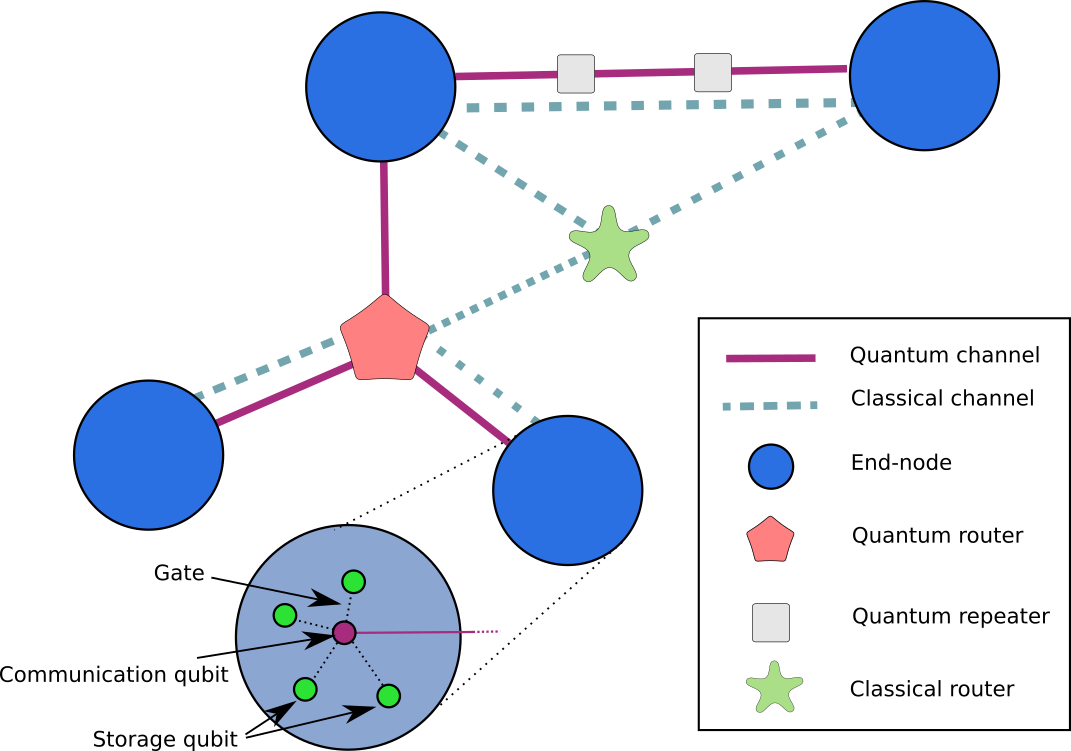
\includegraphics[width=0.4\linewidth]{figures/netqasm/network_model.png}
    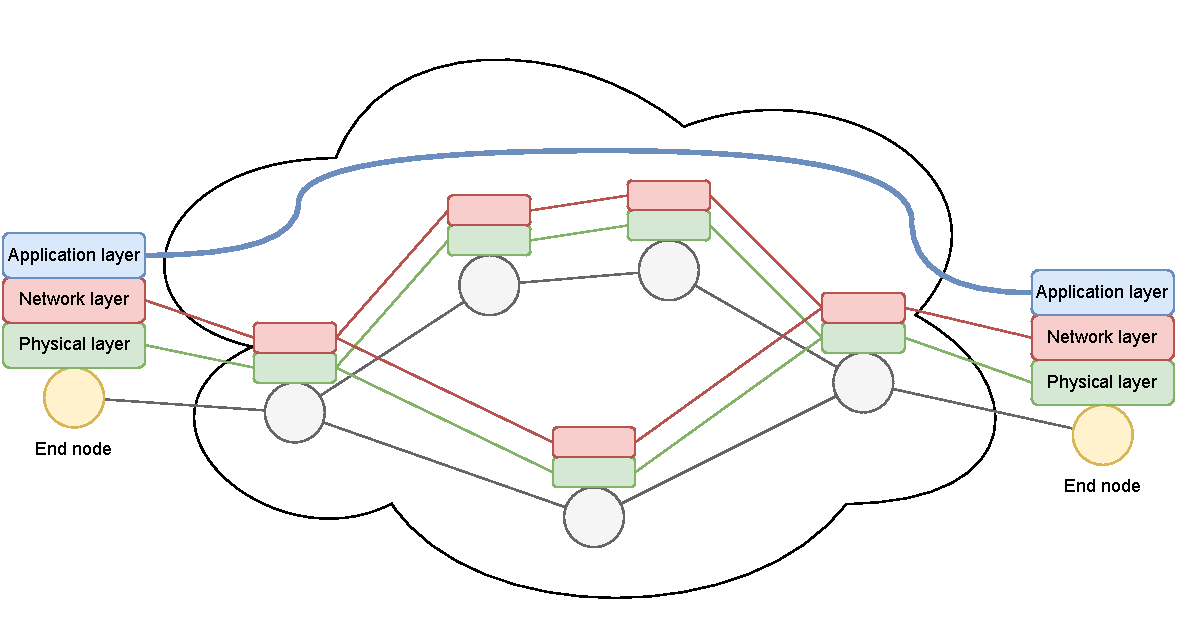
\includegraphics[width=0.8\linewidth]{figures/background/network_nodes.pdf}
    \caption{
        Schematic overview of a quantum network.
        A quantum network consists of nodes (yellow and grey circles) that are connected by classical and quantum communication channels (grey lines).
        Each node implements a physical layer (green boxes and lines) that enables entanglement generation between neighboring nodes.
        % The physical layer is the domain of the QDevice.
        Each node implements a network stack including a network layer (red boxes and lines, which may be subdivided into a separate link layer and a network layer~\cite{dahlberg_2019_egp, kozlowski_2019_towards}).
        This layer realizes long-distance entanglement creation between nodes, and may include protocols such as entanglement swapping and distillation.
        % As QNodeOS implements a network stack, it can also be deployed on intermediary nodes in the network, where e.g. entanglement distillation could be added to the protocol realizing the network layer service implemented by QNodeOS.
        \newline
        We emphasize that the focus of this work is to program and execute applications on the end nodes, i.e. enabling the application layer in networking terms.
        Only \emph{end nodes} (yellow circles) implement an additional application layer (blue boxes and line), which executes arbitrary user applications.
        From the perspective of this layer, end nodes are logically directly connected (blue line) and this layer is hence independent from implementations and protocols in the network layer, and is only dependent on the service  provided by the network layer.
        Logically directly connected means that the application layer relies on the service of the network layer to enable end-to-end entanglement generation between end nodes, and no longer needs to concern itself how the entanglement is generated.
        This abstraction is a key element enabled by a quantum network stack such as~\cite{dahlberg_2019_egp}, and exactly analogous to similar abstractions used in classical networking, where e.g. a web browser can be executed on a laptop independently of how the internet connection between the laptop and a web server is realized.
        % In the same way, QNodeOS can in fact operate also on end nodes separated by a large quantum network of the future, in which many intermediary nodes may lie on the path connecting the end nodes.
    }
    \label{fig:network_model}
\end{figure}

\subsection{Quantum end nodes}
As mentioned above, end nodes in a quantum network possess a quantum processor acting on quantum memory.
These processors differ from classical processors in a number of ways.
Firstly, quantum memory has limited lifetime, meaning that its quality degrades over time.
For example, quantum memories based on nitrogen-vacancy (NV) centers in diamond have impressively been optimized to achieve lifetimes in the order of seconds~\cite{Abobeih2018};
however, this is still very short compared to classical memories, which generally do not have a limited lifetime at all.
Therefore, the quality of program execution is time-sensitive.
Secondly, physical devices are prone to inaccuracies which lead to decreased quality of (quantum) computation.
For example, applying an operation (like a gate) on a qubit affects that qubit's quality.
We note that the two challenges mentioned so far are also inherent to non-network quantum processors.
Quantum \textit{network} processors have additional challenges:
    (1) the processor may have to act as a local computation unit and a network interface at the same time;
    for example, in NV centers, an electron spin qubit is used for generating entanglement with a remote node but is also needed to do local two-qubit gates,
    (2) remote-entanglement operations may not have a fixed time in which they complete, which makes scheduling and optimization more difficult.

Each quantum memory has a certain \textit{topology} that describes which operations can be applied on which (pair of) qubits.
Some of the qubits in a quantum memory may be used to generate an entangled state with another node.
These qubits are called \emph{communication qubits}~\cite{dahlberg2019linklayer}, in contrast to \emph{storage qubits} which can only directly interact with other qubits part of the same local node.
A storage qubit may however hold a state that is entangled with a qubit in another node: after remote entanglement generation using a communication qubit, the state in that local qubit could be transferred to one of the storage qubits, preserving the remote entanglement.
Some platforms only have a single communication qubit and multiple storage qubits~\cite{Bernien2014}, whereas others can have multiple communication qubits~\cite{Inlek2017}.
Quantum processors in general offer two types of qubits (see e.g.~\cite{dahlberg_2019_egp}): \emph{communication qubits} which can be used to generate entanglement with remote nodes next to other quantum operations, as well as \emph{storage qubits} which cannot be used to generate entanglement and only for implementing local quantum operations.
We remark that on near-term quantum processors, the types of operations also depends on the connectivity of the qubits.
That is, not all (pairs of) qubits may allow the same set of quantum operations to be performed on them.

\paragraph{Noise and decoherence}
\todo{elaborate}
Qubits are sensitive to \emph{decoherence} and have limited lifetimes.
Therefore, the timing and duration of operations (such as local gates or entanglement generation with another node) have an impact on the quality of quantum memory. Classical processors control the quantum hardware, and also perform classical computation.
Finally, classical links exist between nodes for sending classical messages.

Since end nodes can control their memory and entanglement generation, they can run arbitrary \textit{user programs}.
End nodes can both communicate classically and generate entanglement between each other, either directly or through repeaters and routers, (\cref{fig:network_model}). Nodes in the network other than end nodes, such as repeaters and routers, do not execute user programs; rather these run protocols that are part of some level in the
network stack~\cite{dahlberg2019linklayer,kozlowski2020networklayer}.
These internal nodes in the network perform elementary link generation and entanglement swapping in order to generate long-distance remote entanglement between end nodes~\cite{dahlberg2019linklayer}.

\paragraph{Hardware implementations}
There are various quantum hardware implementations for quantum network processors, such as nitrogen-vacancy centers in diamond~\cite{Bernien2014}, ion traps~\cite{moehring2007entanglement}, and neutral atoms~\cite{hofmann2012heralded,ritter2012elementary}, which all have different capabilities and gates that can be performed.

\subsection{Quantum processing}
Quantum computing consists of performing operations on quantum bits (qubits).

\paragraph{Circuits and gates}
A quantum program is typically represented as a \emph{quantum circuit}.
\Cref{fig:example_circuit} shows an example circuit of 2 qubits.

\begin{figure}[t]
    \centering
    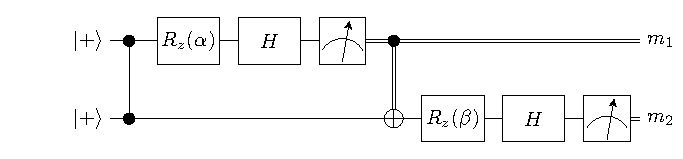
\includegraphics[width=0.8\linewidth]{figures/background/example_circuit.pdf}
    \caption{
      Example circuit of 2 qubits (horizontal lines).
      \todo{elaborate}
    }
    \label{fig:example_circuit}
\end{figure}


A quantum circuit describes the operations that are to be performed on the quantum memory consisting of individual qubits.
Operations include quantum gates (rotation gates or Hadamard), initialization, and measurement (readout).
Quantum gates may be on a single qubit, or on multiple qubits.
For example, the CNOT gate is a 2-qubit gate.

The code, or the `recipe` of quantum programs is hence classical.
The information and memory that the program manipulates is quantum.
Besides quantum operations, there may be limited classical control, such as a gate being executed depending on a measurement outcome.
Typically, a quantum circuit is executed in one go, on a very small timescale.
Quantum memory used for quantum computing \todo{cite hardware platforms} often only stays coherent (alive and useful) for microseconds.

\paragraph{Hybrid classical-quantum processing}
Hybrid classical-quantum programs are used to realize e.g. \textit{variational quantum eigensolvers (VQE)}~\cite{diadamo2021distributed, liu2022layer} or \textit{quantum approximate optimization algorithms (QAOA)}~\cite{farhi2014quantum}.
For such programs, a quantum circuit is executed, followed by some classical processing, and a next circuit is issued.

\subsection{Entanglement generation}
In order for two neighboring quantum network nodes to produce heralded entanglement between them, they need to simultaneously perform an action to trigger entanglement generation (at the physical layer, \emph{synchronized to nanosecond precision}).
This means neighboring quantum network nodes need to perform a network operation (entanglement generation) in a \emph{very specific} time slot in which they make an attempt to generate entanglement.
Such time slots are generally aggregated into larger time bins, corresponding to making batches of attempts in time slots synchronized at the physical layer.
We refer to e.g. Ref.~\cite{pompili_2022_experimental} for background information on the physical layer of entanglement generation in quantum networks, and the readers with a background in computer science to e.g. Ref.~\cite{dahlberg_2019_egp} for a detailed explanation of scheduling of entanglement generation in quantum networks.

In short, network operations in quantum networks need to be executed by the node at very specific time bins.
These time bins cannot be determined by the quantum node itself.
Instead selection of time bins for a specific quantum operation require agreement with the neighboring node~\cite{dahlberg_2019_egp} (and more generally with the quantum network when the end-to-end entanglement is made via intermediary network nodes) by means of a network schedule, e.g. determined by a (logically) centralized controller, see Ref.~\cite{skrzypczyk_2021_arch}.

\paragraph{Quantum network stack}
A quantum network stack has been proposed~\cite{dahlberg2019link} and implemented~\cite{pompili2022experimental} that turns entanglement generation into a robust service independent of the quantum hardware platform.
Important for the design of an architecture for the execution of quantum internet applications is that in this stack, the nodes will establish a network schedule of time slots in which they will trigger entanglement generation (due to need to synchronize entanglement generation at the physical layer~\cite{dahlberg2019link} at high-precision (ns)).
This means that once entanglement has been requested from the network, the nodes can use only the slots in the network schedule to produce entanglement between them, imposing constraints on the ability to schedule applications. What's more, in present day systems~\cite{pompili2021realization, krutyanskiy2023entanglement} limitations in the physical devices prohibit the execution of local operations while engaging in network operations (entanglement generation), creating further dependencies between the local quantum execution and entanglement generation. 
As the specifics of network scheduling~\cite{network-scheduling, skrzypczyk2021architecture} are not within scope of this thesis,
we assume the existence of a \textit{network controller} that takes application demand for entanglement and issues a network schedule to the nodes. 
A schedule consists of sequential time slots, each with a start time and duration, when the node will trigger entanglement generation.
Nodes are not forced to attempt entanglement in corresponding time slots, and can instead choose to do local processing instead.



\section{Quantum network applications}
Quantum network \textit{applications}, also called \textit{protocols}, are multi-partite programs that involve entanglement generation and classical communication between different end nodes, as well as local computation.
Examples include Quantum Key Distribution (QKD)~\cite{bb84, ekert1991quantum}, leader election protocols~\cite{kobayashi2014simpler, ganz2009quantum}, and Blind Quantum Computation (BQC)~\cite{Wehner2018stages}.
In this thesis, we consider quantum network applications in the quantum memory stage~\cite{wehner_2018_stages} and above. That is, applications that require the use of a quantum processor that can manipulate and store quantum bits (qubits). For simpler applications in the prepare-and-measure and entanglement generation stages~\cite{wehner_2018_stages}, e.g. quantum key distribution~\cite{bb84Original,ekert_1991_e91}, where the quantum states are immediately measured by the nodes, it would be sufficient to realize a system implementing a quantum network stack and classical processing only.

\subsection{Programs}
Throughout this thesis, we will use the following terminology.
Applications refer to multi-node protocols or use-cases of quantum networks, such as QKD, BQC, etc.
Programs refer to the code that is run on individual quantum network nodes.
Applications are realized by the joint execution of programs on their respective nodes.

A multi-node quantum internet application is hence partitioned into separate single-node \textit{programs} (e.g. a client program and a server program in BQC) that run concurrently on different network end nodes.
To support security sensitive applications, each program performs local classical and quantum computations on its own private node, and programs interact with each other only via classical message passing and entanglement generation.
This is in sharp contrast to distributed quantum computing (see e.g.~\cite{cacciapuoti2019quantum}), where all nodes can be accessed and controlled by a single program. 


Such applications are split into distinct \textit{programs} each of which runs on a separate end node.


\paragraph{Program ingredients}
% unit of information: bit vs qubit}
% unit of instruction still classical in quantum computing

The single-node programs that constitute a quantum internet application are hybrid in nature (see Fig~\ref{fig:program_illustration}):
First, they contain quantum operations, such as local quantum gates and measurements (e.g. to perform a server computation in BQC), and entanglement generation (e.g. to produce key in QKD). Entanglement is a special property of two quantum bits (qubits) that forms a key resource for quantum internet applications. 
All quantum operations are executed on quantum processors that can store, manipulate and measure quantum information, where small networks including such processors have been realized using different quantum hardware platforms including, for example,  Nitrogen-Vacancy (NV) centers in diamond~\cite{pompili2021realization}, and Ion Traps~\cite{krutyanskiy2023entanglement}.
Second, programs need to perform classical operations, such as message passing (e.g., a BQC client program sending desired measurement bases to the BQC server), and local classical processing (e.g., post-processing measurement outcomes in QKD).


A program is a series of instructions to be executed by a node.
Instructions can be categorized into four types: local classical processing, classical message-passing, quantum local processing (quantum operations), and remote entanglement generation.
A program can keep classical variables in a classical memory, and quantum variables (qubits) in the node's quantum memory during the execution.
Multiple programs, each running on their own node, together form an \textit{application} (see~\ref{fig:program_illustration}), e.g. QKD (two programs, one per node),
or secret sharing~\cite{hillery1999quantum} (a program each on many nodes).
Programs may involve asynchronous operations (e.g. a server awaiting entanglement with multiple clients).


Classical blocks of code consist of instructions for local classical operations and classical message passing. Quantum \emph{blocks of code} consists of
%
\begin{inlinelist}
\item quantum operations (initialization, quantum gates, measurement), 
\item low-level classical control logic (branching on classical variables and loops), as well as 
\item instructions to make entanglement between remote nodes. 
\end{inlinelist}
%

\paragraph{Interactivity}
Classical blocks of code may depend on quantum ones via classical variables generated during the quantum execution (such as measurement results, notification of entanglement generation, and information on the state of the quantum system such as the availability of qubits).
Similarly, quantum blocks may depend on variables set by the classical blocks (such as messages received from remote network nodes).
Finally, quantum blocks may themselves depend on other quantum blocks via qubits in the quantum memory. 

The programs consist of both local operations (classical and quantum) and network operations (classical and quantum), see \cref{fig:app_programs}.
That is, the programs communicate either by passing classical messages, or by establishing quantum entanglement.
For example, BQC involves a \textit{client} node and a \textit{server} node, both of which run their own program.
Their joint execution looks roughly as follows:
    (1) The client and server engage in remote entanglement generation such that the server's quantum memory ends up being in a certain state,
    (2) the client sends instructions to the server in the form of a classical message,
    (3) the server performs a measurement-based computation on its own quantum memory based on the client's instructions,
    (4) the server sends measurement results back to the client,
    (5) the client sends new instructions based on the measurement results,
    (6) repeat steps 3 to 5 until the client obtains its desired result.

The example above illustrates that quantum network programs consist of different
types of operations.
Indeed, program code consists of \textit{classical code}, containing local classical operations and classical communication with other nodes, and \textit{quantum code}, which are operations on quantum memory (such as \textit{gates}) and remote entanglement generation.
Blocks of these types of code may depend on each other in multiple ways, as depicted in~\cref{fig:program_decomp}.
Programs with mixed classical and quantum operations have also been called \textit{dynamic quantum circuits}~\cite{cross2021openqasm, burgholzer2021towards}, but these do not cover the networking dimension found in programs we consider here, such as the dependency on remote information and entanglement generation operations.

Due to the nature of quantum network programs, execution may have to \textit{wait} for some time. For example, the program needs to wait until another node sends a classical message, or until remote entanglement has been established.
Therefore, it makes sense to run multiple (independent) quantum network programs on a node at the same time (interleaved), so that processor idle times can be filled by execution of other programs. This is something that typically does not happen on local quantum computers, and therefore introduces new challenges.

\paragraph{Independence of programs}
Quantum network applications may be programmed by a single actor.
For example, a developer may program a QKD application in the form of a two programs, and distribute these two programs to two end nodes in the network.
Alternatively, a single-node quantum network program may be developed separately from other programs, possibly not knowing how these other programs are implemented.
For example, a BQC service provider could have already implemented the server-side program of a specific BQC protocol.
A client may then write the client-side of this protocol, without having control over the server-side implementation.



\subsection{Application execution}

\paragraph{Mode of Execution}
There exist quantum applications and functionalities, where one pair of programs is executed only once, e.g. a simple example of quantum teleportation~\cite{bennett_1993_teleportation}.
As in quantum computing, however, some quantum network applications~\cite{wehner_2018_stages} are expected to succeed only with a specific \emph{probability of success} $p_{\rm succ}$ when executed once.
In many quantum internet applications (e.g. BQC), a single execution of the application can result in failure or success (e.g. a BQC client receives correct measurement results from the server program~\cite{leichtle2021verifying}).
Quantum internet applications have classical outcomes that are typically probabilistic in nature:
(1) applications may intentionally do measurements on quantum states that have fundamentally probabilistic outcomes (e.g. quantum cryptography),
(2) in practice, quantum hardware is imperfect (or \textit{noisy}). That is, undesired errors occur
when performing operations (such as gates, measurements, or entanglement generation) or when keeping quantum states in memory for too long.
Applications are often executed many times, where outcome statistics are computed in order to validate successful execution (e.g. by majority of outcomes).
The application is then typically executed many times in succession in order to gather statistics (for example to amplify $p_{\rm succ}$).


\paragraph{Performance metrics}
Performance of application execution on quantum network nodes can be measured by several metrics.
In this thesis we consider metrics that either apply to a single application that one executes on the quantum network, or on a node in the network that executes one or more applications.

For an application, we consider \textit{makespan} as a classical metric and \textit{success probability} as a quantum metric.
Makespan is the time it takes to execute (all repetitions of) the application.
The success probability is the one mentioned above.
It is typically related to quantum fidelity $F \in [0, 1]$, which is a measure of closeness of a quantum state to some ideal quantum state.
Noisy quantum systems produce non-perfect quantum states ($F < 1$) which decrease application success probability.
For quantum network nodes, we consider common classical metrics~\cite{stankiewicz_commag}\todo{better refs}: utility (fraction of time that a node is doing useful things), throughput (amount of application executions per time unit) and latency (which may be between internal components of a node, or between nodes).




\begin{xstretch}
\printbibliography[heading=subbibintoc,title={References},notcategory=noprint]
\end{xstretch}
